\documentclass{bioinfo}
\usepackage{float}
\copyrightyear{2022} \pubyear{2022}
\access{Advance Access Publication Date: Day Month Year}
\appnotes{Manuscript Category}

\begin{document}
\firstpage{1}

\subtitle{ECSE 552 - Deep Learning}

\title[SeqRec]{SeqRec: A Deep Learning Based Recommendation System for Sequential Data}
\author[Group 10]{Group 10: Safyan Memon, William Ma,
Yazdan Zinati,
Sohaib Jalali,
Mai Zeng,
and Yuxiao Liu}
\address{McGill University, Montreal, Canada}

\corresp{$^\ast$To whom correspondence should be addressed.}

\history{Received on XXXXX; revised on XXXXX; accepted on XXXXX}

\editor{Associate Editor: XXXXXXX}

\abstract{\textbf{Motivation:} Recommendation systems are used by major services like YouTube, Netflix and Amazon to recommend items or content of interest to their users. Sequential patterns in data play a significant role in how well a recommendation system performs. However, the struggle to uncover complex sequential relationships in a user’s history is still common.\\
\textbf{Results:} In this study, we propose a deep learning based approach that utilizes the user's history. Using a multiplicative long short term memory (mLSTM), we capture the sequential information of a user. On the MovieLens 1M dataset of 6040 users and 3706 movies, resulting in over a million interactions, we trained a deep learning network to capture the sequential information of each user by utilizing the user characteristics, the item features and the user-item history. Our highest reported Mean Squared Error (MSE) was 0.958. \\
\textbf{Availability:} The dataset and code is available at https://github.com/YazdanZ/SeqRec\\
\textbf{Contact:} \href{safyan.memon@mail.mcgill.ca}{safyan.memon@mail.mcgill.ca}\\
}

\maketitle

\section{Introduction}

The impact of COVID-19 on the rise of e-commerce was unprecedented. Businesses that had never found the need to set up online stores were in dire need of online systems to keep their businesses afloat. With the rising demand of new e-commerce platform came easy to implement and use recommendation systems \citep{ricci2011introduction}. A recommendation system is a type of information filtering system used to predict the preference a user might give to an item by analyzing user's history and interests, or by comparing the similarity with other neighbouring users.

In simple terms, it is an algorithm which suggests relevant items to a user. They aid in decision making as they help users make informed buying decisions based on their preference, buying patterns or browsing history.

We see recommendation systems everyday. Whether it's on an e-commerce website such as amazon or a music/movie streaming platform such as Spotify or Netflix, our interactions with platforms that employ these systems is endless. We can categorize recommendation systems into two main categories: \textit{collaborative based} filtering and \textit{content based} filtering \citep{balabanovic1997fab}.

\textit{Collaborative based} filtering systems use prior historic interactions between the user and the items to produce new recommendations, with the idea being that the past-user item interactions are sufficient to detect similar items and make predictions on these estimated proximities. The interactions between the user and the item are stored in an aptly named "user-item interaction matrix". Amazon is the most infamous example of a collaborative-based filtering system. It not only works on a user's purchase history but also takes into account the items that a user views more frequently than others.

%Collaborative systems have the advantage of requiring no information about the user or the item, making them easy to use in many situations. As only the interaction between user and item is recorded, the more users interact with items the more new recommendations become accurate: for a fixed set of users and items, new interactions recorded over time bring new information and make the system more and more effective.

As collaborative systems consider past interactions to make predictions, they cannot recommend anything to new users. This is known as the "cold start problem" \citep{lam2008addressing}. To mitigate this problem, a non collaborative based method can be used which does not need to take into account a user's history.

\textit{Content based filtering} systems use information about the user or the item to predict a users preference, unlike the collaborative filtering approach, which only rely on the user-item interactions. These systems try to build a model using the available "features", which explain the interactions between users and items. If one type of user rates an item better than others, then that item will be recommended by the models to similar type of users. 

These methods suffer far less from the cold start problem than collaborative approaches as new users or new items are described by their characteristics and so relevant suggestions can me made for new entities. Only new users or items with previously unseen features suffer from this drawback, but once the system is old enough, the chances for this problem occurring are minuscule. The music streaming platform, Spotify adapts a combination of content and collaborative based filtering to recommend new music to its users. 
%\subsection{General Recommendation}
% Wang et al. worked based on calculating prediction ratings and generating recommendation lists. Both Long-short term memory network (LSTM) and CNN were used for experiments in their work and the dataset is MovieLens 1M. LSTM is improved from recurrent neural network (RNN). 

The high demand of recommendation systems has resulted in a significant increase in new approaches using machine learning to build better and faster tools. Here, we explore a few of the important and recent approaches in this field. There are two types of recommendation systems that we focus on in this study: \textit{general recommendation} systems and \textit{sequential recommendation} systems.

\textit{General recommendation} systems are used for modeling the relationships between users and items given the history of the user-item interactions. User feedback is normally divided into 2 ways, explicit way (ratings) and implicit way (clicks, purchases, comments). Modeling implicit feedback is challenging since this approach has to explore the latent data (not directly observed). To cater to this problem, pair-wise methods are usually used \citep{pairwise}.

\textit{Matrix Factorization (MF)} methods are usually used to seek this latent dimensions representing users' preferences and items' properties too. Through the inner product between the user and item embedding the interactions between the user and items can be estimated. Furthermore, \textit{Item Similarity Models} (ISM) were used to model user with the latent factors \citep{FISM}. FISM learns an item-to-item similarity matrix and then estimate the user's preference toward an item by measuring its similarities with items that the user has interacted with.

Several deep learning based recommendation systems were introduced by \citep{DLRecomSys}. The deep neural networks are able to extract the user and item features. Based on this, several deep learning techniques are designed to replace the conventional MF methods. NeuMF \citep{NeuMF} estimates user preferences through Multi-Layer Perceptions (MLP). AutoRec \citep{AutoRec} is to predict the ratings with autoencoder technique. 

%\subsection{Sequential Recommendation}

\textit{Sequential recommendation} systems, which usually mainly work using the foundations of collaborative based filtering, aim to model sequential patterns among successive items for a user. Many methods are based on modeling the item-item transition matrix. Because the last visited item is often the key factor affecting the user's next action, the first-order Markov Chain (MC) based methods can be used to capture transition matrix \citep{MC_based_rec}. Several methods which adopt the high-order MCs (considering previous items) also gave some promising results \citep{High_order_MC_Rec}.

Convolutional Neural Networks (CNN) are able to capture the patterns in a sequence of data too. The CNN based method Convolutional Sequence Embedding (Caser) treats the embedding matrix of $L$ previous items as an "image" and applies convolution to extract the transitions \citep{Caser}. 

Although Caser is able to capture the sequence pattern, due to the model's capacity CNNs still cannot perform that well on sequential data. Recurrent Neural Networks (RNNs) are good for modeling the sequence data therefore, RNN-based methods are adopted in the sequential recommendations a lot. RNNs take the state from the last step and current action as its input for each time stamp. Methods like GRU4Rec \citep{GRU4Rec} take advantages of Gated Recurrent Units (GRUs) to model the sequences and an improved version boosts its Top-N recommendation performance \citep{Top_K_Booster_GRU}

% Maybe remove this section if word issue

%\subsection{Session-based Recommendation}
%The session-based recommendation system (SBR) is based on chronologically ordered or unordered user-item interactions that happen together in a continuous period of time \citep{sbr_survey}. The Matrix Factorization (MF) methods mentioned in Section 1.1 are hard to apply in session-based recommendation due to the absence of a user profile. On the other hand, ISM have been used extensively in session-based recommendations \citep{sbr_rnn}. However, the issue with the latter method is that it only account for the last click of the user and ignores historical information. Markov chains can be used to train SBR models, with the issue that that the state space quickly becomes unmanageable when trying to include all possible sequences of user selections \citep{sbr_mdp}.
%Graph Neural Networks (GNN) is able to model the complex transitions within or between sessions. Session dataset is firstly transferred to a graph $G$ by mapping each session into a chain on the graph before feeding into GNN. Pioneering work includes SBR with Graph Neural Networks (SR-GNN) \citep{sbr_gnn}, which claimed to have achieved superior performance, compared with non-GNN approaches.
%Generative Model(GM) generates next interaction(s) in SBR problems using a generation process. This can be a probabilistic generative model as proposed in \textit{NextItNet} that was devised to generate a probability distribution over the candidate items \citep{sbr_survey}. In general, GM can be applied to problems with dynamic and incremental sessions, with the advantage of modelling closely to the session information.

\subsection{SeqRec}

%query (movie, user) pair.
%user's movie rating history

Keeping in mind the existing recommendation systems which utilize the sequential information of data, we introduce our approach, SeqRec which utilizes the sequential information from the MovieLens dataset \citep{harper2015movielens} to recommend new movies of interest to the user. This deep-learning based approach predicts the rating of new movies that a user might give based on the user's movie rating history. This sequential information is captured by  an mLSTM \citep{krause2016multiplicative}. The features related to the user and movie are captured by feed-forward neural networks (FFNNs) and a tranformer \citep{vaswani2017attention}. The architecture achieved a root mean squared error (RMSE) of 0.958. Along with this, we round off each prediction and compare it with the true value thus turning the regression task into a classification task. With this new task, we achieved an accuracy of 0.397.  


%Keeping in mind the existing recommendation systems which utilize the sequential information of data, we introduce our approach, SeqRec which utilizes the sequential information from the MovieLens dataset \citep{harper2015movielens} to recommend new movies of interest to the user. This deep-learning based approach predicts the rating of new movies that a user might give based on the past ratings they have given to the movies they have interacted with. Using a network that comprises of an mLSTM \citep{krause2016multiplicative}, a transformer \cite{vaswani2017attention}, and feed forwards neural networks, we achieve a mean squared error of 0.958. Along with this, we round off each prediction and compare it with the true value thus turning the regression task into a classification task. With this new task, we achieved an accuracy of 0.397.  

\begin{methods}

\section{Methods}

\subsection{Dataset}

We are using the MovieLens 1M dataset to train and benchmark our model \citep{harper2015movielens}. This dataset contains nearly 1 million interactions between 6040 users and approximately 3706 movies. User-movie interactions are given a 1-5 stars rating and a timestamp corresponding to the time of the rating. The timestamp of the interaction allows us to create a sequential recommendation system. Additionally, the dataset provides us with information about users who take part in interactions, which we take advantage of. This information includes age group, occupation and sex. For movies, we are provided with movie titles and genres. Aside from the sequential nature of interactions, and information about entities taking part in them, we chose this dataset as it has become a benchmark dataset for recommendation systems, allowing us to compare the performance of our method with existing works.

Nonetheless, the dataset possesses traits that render deep learning work on it challenging. As shown in Figure \ref{fig:dataset} (a), ratings are unequally distributed between the five available stars. For instance, the dataset contains nearly 7 times more interactions with a 3-star than 1-star ratings. Imbalances do not end at ratings since the distribution of reviews per movie and movies per user is also highly imbalanced. As it can be seen from Figures \ref{fig:dataset} b and c, a few movies receive substantially more ratings than others and some users have rated many more movies than others. These imbalances pose challenges by biasing models trained on this dataset towards specific ratings, movies, or users. Table \ref{tab:dataset} contains further details, highlighting some of the mentioned imbalances in the dataset. 

\begin{figure*}[h]
    \centering
    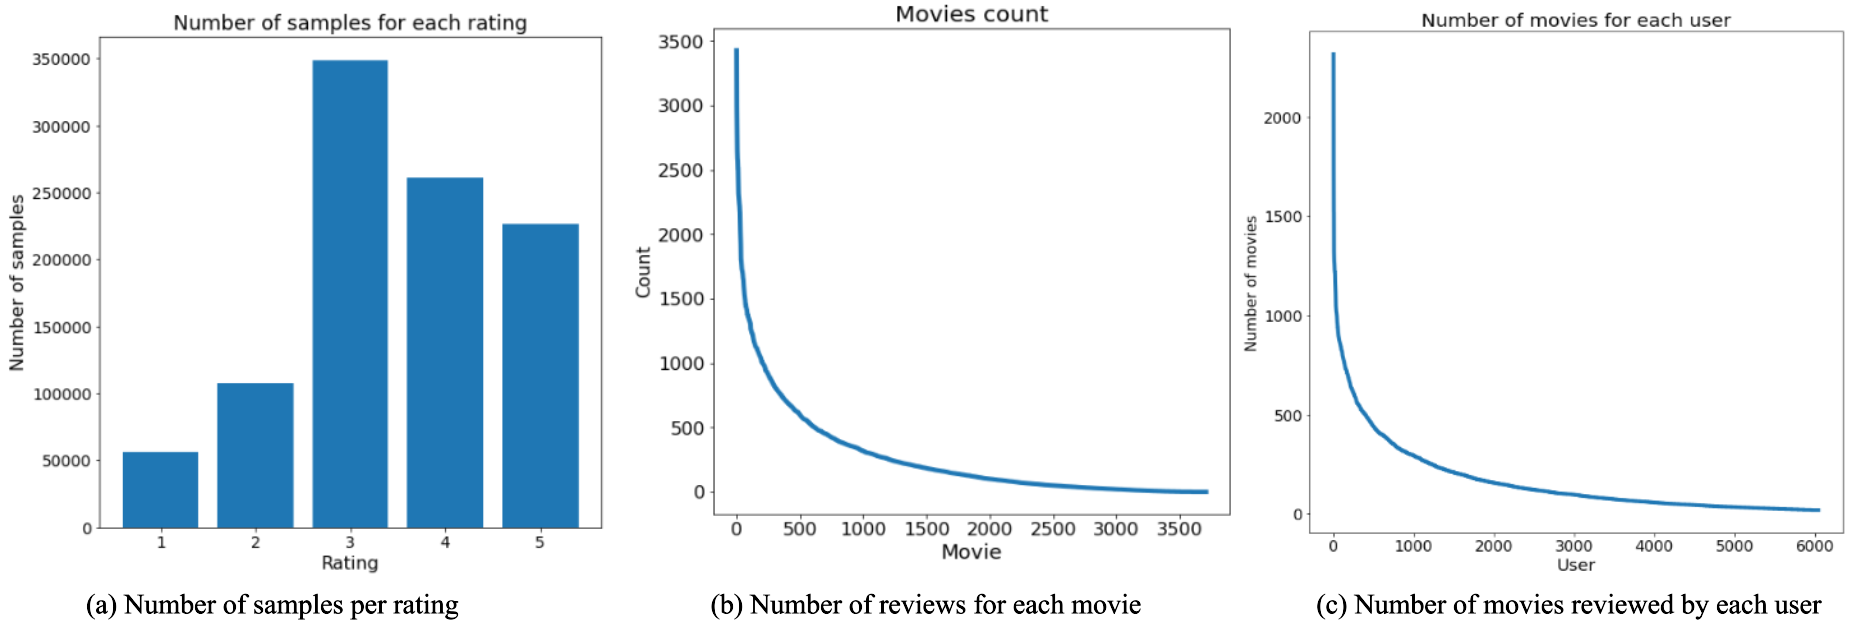
\includegraphics[width=\textwidth,height=0.33\textwidth]{figures/dataset.png}
    \caption{Characteristics of the MovieLens 1M dataset}
    \label{fig:dataset}
\end{figure*}

\begin{table}[h]
\begin{tabular}{|l|l|l|l|l}
\cline{1-4}
Data characteristic &  Minimum & Maximum & Mean &  \\ \cline{1-4}
Rating & 1 & 5 & 3.49 &  \\ \cline{1-4}
Number of movies reviewed by users & 20 & 2314 & 356.6 &  \\ \cline{1-4}
Number of reviews per movie & 1 & 3428 & 269.8 &  \\ \cline{1-4}
\end{tabular}
\caption{Characteristics and imbalances of the MovieLens 1M dataset }
\label{tab:dataset}
\end{table}

\subsection{Data processing}

Each sample is an interaction, designed as a (user, movie) pair with a rating as the label. For both users and movies, we incorporate multiple data modalities as features.

A unique \textit{movie ID} is directly passed into the model, and the \textit{movie genre} was encoded in multi-label binary format with each of 18 genres as features. The \textit{movie title} was directly passed as a string into the model. These formed the data modalities

\textit{User information} includes age, sex, occupation. Age is composed of 7 discrete age groups ranging from 'under 18' to '56+', which we encoded as a scalar of the minimum of each age group. Sex and occupation are composed of 2 and 21 categories each, which are one-hot encoded. The user information is concatenated into a vector of length 24.

A challenge was how to incorporate a given \textit{user history} of movie ratings. As interactions for a given user are also samples, we separated each user's set of movie ratings, reserving the first 50\% of sorted movie ratings as a user's sequential ratings history, with the latter 50\% used as samples. The choice of 50\% as the cutoff was chosen as a trade-off between sparsity of samples and the user's history of preferences, as well as the average time between the most recent interaction for a given user and the query interaction pair. For each user, the history was formatted as an ordered sequence of movie IDs and their corresponding ratings.

To prevent data leakage, we split the data based on each of the 6040 users into training, validation, and test sets of 80\%, 10\%, and 10\% respectively. As the number of ratings varied by user, the resulting percentage of samples in each set were not exactly the same as the proportions of the split; they were 407,929, 45,612, and 45,082 for the training, validation, and test sets, respectively.

\subsection{Model}

Our model consists of multiple branches for the different data modalities of a query (movie, user) pair.

To capture the sequential nature of a user's movie rating history, we used a multiplicative LSTM (mLSTM) \citep{krause2016multiplicative}. An mLSTM possesses all the features of a regular LSTM and works in a similar way with the addition of the hidden states being able to react to unexpected inputs. Figure ~\ref{fig:mlstm} shows a single cell of an mLSTM.

\begin{figure}[h]
    \centering
    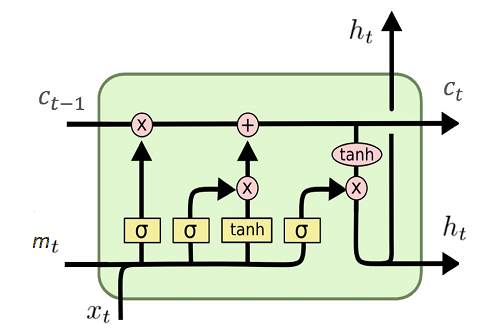
\includegraphics[width=\columnwidth]{figures/mlstm.png}
    \caption{An mLSTM cell.}
    \label{fig:mlstm}
\end{figure}

A regular LSTM has the input of {${h_{t-1}}$} instead of {$m_{t}$}. {${h_{t-1}}$} refers to the previous input. We can see below the definition of this new input:

\begin{equation} \label{mlstm_equation}
m_t = (W_{im}x_t + b_{im}) \odot (W_{hm}h_{t-1} + b_{hm}),
\end{equation}

% {${\hat{Y}}$} 

where {${W}$} represents the weights, {${b}$} are the biases and {${h_{t-1}}$} is the previous hidden state.  

The mLSTM incorporates the movie rating history of a user which is a single branch called the \textbf{user history} branch in our network. For each element, the \textit{movie ID} is encoded using a learnable embedding, which is then concatenated with the rating, and the sequence is passed into the branch to produce a representation.

In addition to the \textit{user history} branch, there are three other branches in the network. The four branches are:
\begin{enumerate}
    \item user history
    \item user information
    \item movie information (ID and genre)
    \item movie
\end{enumerate}
with 1 and 2 representing the user and 2 and 3 representing the movie in the query pair. Figure ~\ref{fig:model} shows the entire architecture of SeqRec.

\begin{figure*}[h]
    \centering
    \includegraphics[width=\textwidth,height=85mm]{figures/model2.png}
    \caption{The model architecture for SeqRec.}
    \label{fig:model}
\end{figure*}

The \textbf{user information} branch is a FFNN, to which the \textit{user information} vector is passed.

The \textbf{movie information} branch is also a FFNN. Parameter sharing is exploited by using the same embedding encoding in the mLSTM to encode \textit{movie IDs}, which is then concatenated with the \textit{movie genre} before being passed into the branch.

For the \textbf{movie title} branch, the \textit{movie title} is first encoded using a transformer architecture \citep{vaswani2017attention}, using the pre-trained 'all\-MiniLM\-L6\-v2' model \citep{reimers-2019-sentence-bert}, chosen because it generates a 384 dimension embedding at high speeds with good performance. This is then passed into a single fully connected layer.

The information from each branch is concatenated and passed to a FFNN for the final prediction. Since we treat this problem as a regression task, the loss function is mean squared error (MSE) (see equation 2 in Section 3.1).

The model structure parameters are shown in Table ~\ref{tab:model}.

\begin{table}[H]
\centering
\begin{tabular}{|l|l|l|}
\hline
\textbf{Branch} & \textbf{Parameter} & \textbf{Value} \\ \hline

\textbf{user history} & hidden embedding size & 111 \\ \hline
\textbf{user history}, \textbf{movie information} & movie embedding size & 110 \\ \hline
\textbf{movie information} & layer sizes & [128, 128, 128]\\ \hline
\textbf{user information} & layer sizes & [24, 24, 24]\\ \hline
\textbf{user title} & layer sizes & [192]\\ \hline
\textbf{output} & layer sizes & [227, 227, 1]\\ \hline
 & Activation Function & ReLU \\ \hline
\end{tabular}
\caption{Model structure parameters.}
\label{tab:model}
\end{table}

Alongside this architecture, we trained a network where we replaced the mLSTM component of the network with a regular LSTM to compare the results. Furthermore, as a baseline, we trained a simple 3-layer FFNN and another similar network where the movie titles were passed through the pre-trained 'bert-base-uncased' transformer to create embeddings.

\subsection{Training}
The model was trained using the AdamW optimizer \citep{loshchilov2017decoupled} and a learning rate schedule composed of a warm-up from half the maximum learning rate to the maximum in the first epoch, then annealing across the remainder back to half the maximum learning rate. Early stopping was additionally employed, with the model with lowest validation loss at the end of an epoch chosen as the final model, stopping training if the validation loss failed to improve after 5 epochs. To reduce training time, user histories were cropped to the last 100 samples. The hyperparameters used are shown in Table ~\ref{tab:hyper}.

\begin{table}[h]
\centering
\begin{tabular}{|l|l|l|}
\hline
\textbf{Hyperparameter} &  \textbf{Value} \\ \hline

user history sequence length & 100 \\ \hline
epochs & 20\\ \hline
max learning rate & $5.0 \times 10^{-4}$\\ \hline
batch size & 512 \\ \hline
optimizer & AdamW \\ \hline
weight decay & $1.0 \times 10^{-4}$ \\ \hline
AdamW Epsilon & $1.0 \times 10^{-8}$ \\ \hline
AdamW Betas &  (0.9, 0.999)\\ \hline
FFNN dropout &  0.5 \\ \hline

\end{tabular}
\caption{Hyperparameters used in training.}
\label{tab:hyper}
\end{table}

% William
% Lets talk about the learning rate, epochs, etc.
% As well as we should mention here the configuration of the network. the units in the mlstm. the neurons in the FFNNs etc
% The mLSTM component of the network comprised of XXX layers.


% tell that we are clearly overfitting and talk about how you used dropout to combat that but that didnt work
% talk about future work on overfitting problem. Put the loss on train and test set to prove the point that we're overfitting. 

% Also don't forget to add the loss and accuracy curves here

\begin{figure}[H]
    \centering
    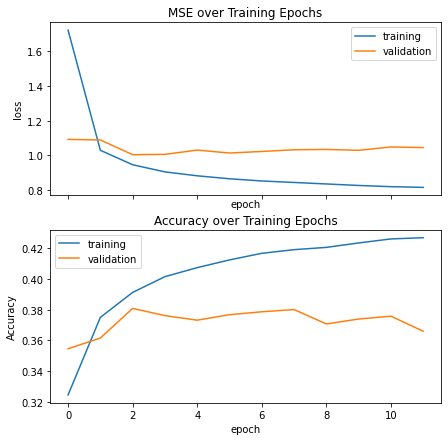
\includegraphics[width=\columnwidth]{figures/results.png}
    \caption{Training and validation MSE and accuracy over training epochs.}
    \label{fig:curves}
\end{figure}


The validation and training loss and accuracy (see equation 3 in Section 3.1) over training are shown in Figure ~\ref{fig:curves}, which indicates overfitting as the validation loss reaches a minimum in 3 epochs, with the training loss rapidly decreasing afterward. This demonstrates the utility of early stopping as a regularization technique, but also the need for further regularization in future work.


\end{methods}

\section{Results}

\subsection{Metrics}

To evaluate our model, we use MSE. The formula for MSE can be found in equation 2:

\begin{equation} \label{mse_equation}
MSE = \frac{1}{n}\sum_{i=1}^{n} (Y_i - \hat{Y})^2,
\end{equation}

where {${n}$} is the total number of samples in a batch, {${Y_i}$} is the true value and {${\hat{Y}}$} is the predicted value.

Alongside the regression task and the use of MSE, we also evaluated our model from a classification point of view. Each prediction (predicted rating) was rounded and compared to the actual rating. Therefore, for this task, we used accuracy as the metric of evaluation. The formulae for accuracy can be found below:

\begin{equation} \label{accuracy_equation}
Accuracy = \frac{True\;positives + True\;negatives}{All\;samples}
\end{equation}

\subsection{Comparison}

We evaluated our model by comparing it to other state of the art recommendation systems. Table ~\ref{tab:results} shows the results.

GLocal-K \citep{han2021glocal} is an approach to predict the ratings of a movie based on an autoencoder architecture and a convolution based global kernel. Similarly, GC-MC \citep{berg2017graph} utilize a graph autoencoder framework based on differential message passing on the interaction graph. Finally, BST \citep{chen2019behavior} uses a sequence transformer to capture the sequential signals underlying users’ behaviors to ultimately construct a recommendation system.

\begin{table}[h]
\centering
\begin{tabular}{|l|l|l|}
\hline
\textbf{Method} &  \textbf{RMSE} & \textbf{Accuracy} \\ \hline
GLocal-K (Autoencoder) & 0.823 & - \\ \hline
GC-MC (graph autoencoder) & 0.832 & - \\ \hline
BST (Transformer) & 0.841 & - \\ \hline
\textbf{Test set standard deviation} & \textbf{1.125} & \textbf{-} \\ \hline
\textbf{3-layer neural network} & \textbf{0.99} & \textbf{-} \\ \hline
\textbf{FFNN + BERT (Movie Title)} & \textbf{0.99} & \textbf{-} \\ \hline
\textbf{SeqRec\_LSTM} & \textbf{0.970} & \textbf{-} \\ \hline
\textbf{SeqRec} & \textbf{0.958} & \textbf{0.397} \\ \hline
\end{tabular}
\caption{A comparison of different machine learning approaches on the MovieLens 1M dataset. The results in bold are the approaches we did. The use of accuracy was only employed in the SeqRec approach by rounding off the predictions and changing the problem into a classification task.}
\label{tab:results}
\end{table}

We constructed four models: a simple 3-layer FFNN, a network which was similar to FFNN but the title of the movie was passed through a transformer architecture to create a learned embedding and finally the two SeqRec approaches where one uses the simple LSTM architecture (SeqRec\_LSTM) and the other uses the mLSTM (SeqRec).

We can see SeqRec performed better than all our other approaches. However, the performance did not outshine the state of the art methods (autoencoders and transformer). To better understand the reason behind the SeqRec's performance, we conducted an ablation study which is explained in the next section.

\subsection{Ablation Study}
To gain a better understanding of our model, and quantify the effect of each component, we performed an ablation study. We followed the approach outlined by \cite{meyes2019ablation} where weights of the ablated branch are set to zero, rendering the branch blind to inputs. Following the ablation, we let the damaged network recover by training it for an additional two epochs with the rates frozen before recording results. The result of this ablation study is shown in Table \ref{table:ablation}.

\begin{table}[H]
\centering
\begin{tabular}{|l|l|}
\hline
\textbf{Ablated Branches} &  \textbf{RMSE} \\ \hline
% Full model &  0.925\\ \hline
% SeqRec $-$ movie\_id & 0.973 \\ \hline
% SeqRec $-$ movie\_title & 0.938 \\ \hline 
% SeqRec $-$ movie\_id and title & 1.181 \\ \hline
% SeqRec $-$ user\_history &  0.944\\ \hline
% SeqRec $-$ user\_information &  0.925\\ \hline
% SeqRec $-$ user\_history and information &  0.951\\ \hline
% SeqRec $-$ movie\_id, title, user\_history and information & 1.171\\ \hline

\textbf{none} (full model) &  0.962\\ \hline
\textbf{movie information} & 0.986 \\ \hline
\textbf{movie title} & 0.968 \\ \hline
\textbf{movie id}, \textbf{movie title} & 1.087 \\ \hline
\textbf{user history} &  0.972\\ \hline
\textbf{user information} &  0.962\\ \hline
\textbf{user history}, \textbf{information} &  0.975\\ \hline
\textbf{all branches} & 1.082\\ \hline

\end{tabular}
\caption{Results on test set of ablation study conducted on SeqRec after 2 recovery epochs.}
\label{table:ablation}
\end{table}

The ablation study shows the full SeqRec model performs the best. Furthermore, we note that the ablation of both movie id and title results in a considerable increase in MSE loss, suggesting their importance. On the other hand, ablation of the branch processing user demographic information does not result in a loss in performance. We will consider processing user information in new ways to increase its role in SeqRec rating predictions. By ablating the user history branch (the mLSTM), we see an increase in MSE implying that sequential information is captured and used by our model for customizing movie ratings to users based on their history. 

It is hard to pinpoint if our model is basing its ratings mainly on the movies rather than on users. A movie is likely to have good or bad ratings solely based on its content and user preference can only have minimal effect on the rating given to the movie. Furthermore, the dataset is biased since users are presumably watching and reviewing movies appropriate to their demographic (age group, sex, occupation).



\subsection{Limitations}

Since the network was quite deep with over xx parameters, a key limitation of this study which prevented us from performing a wide range of experiments was the training time. Another factor was determining the sequence length to use when passing the data to the mLSTM. A longer sequence length would result in better performance but very long training times. In contrast, a shorter sequence length resulted in much faster training but poor performance.

Finally, the data imbalance problem that we saw in Figure 1 could be a reason for the overall performance. The users with the higher number of examples performed significantly better than the users with a few examples. From the data distribution, we saw that only a small fraction of the users have hundreds of thousands of movies.

\section{Conclusion and Discussion}
Our goal for this work was to incorporate the sequential nature of the data which we believed would lead to better results. In this work, we proposed SeqRec, a new recommendation system architecture for incorporating information about the entities taking part in interaction along with their interaction history. To benchmark the proposed architecture, we trained the recommendation system on the Movielens 1M dataset where interactions are between movies and users. An mLSTM is used to learn sequential information while two FFNNs are used to find embeddings for parties taking part in the interaction. In our case, branches corresponded to users and movies and we added a transformer to perform sequence transduction using movie titles. However, this architecture can be applied to new datasets with more entities taking part in an interaction. In that case, new branches could be added to model new entities. 

Using this approach, we achieved an RMSE of 0.958, which falls short when comparing the result to the other state of the art methods (GLocal-K, GC-MC and BST). Unfortunately, due to time and resource limitation, we were unable to improve the model further. A major problem encountered was data imbalance, where some users rated thousands of movies and some only rated a couple and similarly some movies had thousands of user ratings whereas others only had a few, which severely impacted the results obtained.

\section{Future work}

Even though SeqRec has shown its effectiveness on predicting ratings for user-movie pairs while integrating sequential information, we have clear paths to follow to improve upon the existing model. From the ablation study we determined that user information such as demographic had minimal impact on the performance of the model. However, this feature is important, as users' preferences is related closely to their demographic. Considering new architectures for learning user demographic embeddings and providing them to our final FFNN will likely improve SeqRec's performance. 

From the large gap in train and test set performance, we believe our model is overfitting to the data. We combatted this issue by introducing dropout to our model. Even though this mitigated the overfitting issue, still a wide gap exists between train and test performance. To fix the overfitting issue, we first need to pinpoint which of our model's branches are overfitting. Next, we will apply new regularization techniques that are shown to be effective in LSTMs. 

Data imbalance was one of the major issues we faced, which may have contributed heavily in achieving less than ideal results. From Figure 1, which represents the distribution of our dataset, we can observe that some users have reviews of hundreds of movies but most of the users have only reviews of less than a hundred. Similarly, some popular movies have received ratings by thousands of people, whereas most movies were viewed and rated by only a couple hundred of users. This stark difference in the distribution of the data greatly reduces the performance of the model and skews the results. Experimenting with different techniques is key in future attempts to overcome this issue of user loss/balancing.

A worthwhile modification to the model would be to use Graph Convolutions Networks. Adding a GCN to SeqRec would allow us to capture the graphical information in addition to sequential information. Relying on the GCN to capture long term dependencies between the users and their interaction with movies, will allow the use of collaborative filtering methods to recommend similar movies to users with similar taste. This may constitute the object of future studies.

\bibliographystyle{natbib}
\bibliography{ref}

\end{document}